\documentclass[10pt]{beamer}

\usepackage{multicol}
\usepackage[ngerman]{babel} 
\usepackage[T1]{fontenc}

\usepackage{blindtext}
% Zeilenabstände auf 0 setzen
%\usepackage{enumitem}

\usepackage{verbatim}

% Formeln
\usepackage{amsmath,amssymb,amstext,mathabx}

% Schrift
%\renewcommand*\familydefault{\sfdefault}
%\newcommand{\changefont}[3]{\fontfamily{#1} \fontseries{#2} \fontshape{#3} \selectfont}

% Farben
%\usepackage[usenames,dvipsnames]{xcolor}

\usepackage{parcolumns}
\usepackage{pstricks-add}

%Definiere Farben:
\definecolor{orange}{rgb}{1,0.5,0}
\colorlet{notgreen}{blue!50!yellow}
\usepackage{pdfpages}
\usepackage{diagbox}
\usepackage[T1]{fontenc}
\usepackage{algorithm,algorithmic}
\usepackage{float}
\restylefloat{table}


% some other useful packages
%\usepackage{url}


%%%%%%%%%%%%%%%%%%%%%%%%%%%%%%%%%%%%%%%%%%%%%%%%%%%%%%%%%%%%%%%%%%%%%
%%% my shortcuts
%%%%%%%%%%%%%%%%%%%%%%%%%%%%%%%%%%%%%%%%%%%%%%%%%%%%%%%%%%%%%%%%%%%%%
\newcommand{\highlight}[1]{{\color{blue}\bf#1}}
\newcommand{\todo}[1]{{\color{blue}\bf TODO: #1}}


%%%%%%%%%%%%%%%%%%%%%%%%%%%%%%%%%%%%%%%%%%%%%%%%%%%%%%%%%%%%%%%%%%%%%
%%% setup beamer presentation theme
%%%%%%%%%%%%%%%%%%%%%%%%%%%%%%%%%%%%%%%%%%%%%%%%%%%%%%%%%%%%%%%%%%%%%

\mode<presentation>
{
  \usetheme{TUDortmund2}
}

% include intermediate TOCs automatically at each \section
\AtBeginSection[]
{
  \begin{frame}[c]
    \frametitle{Content}
    \tableofcontents[currentsection]
  \end{frame}
}

% Suppress navigation symbols
\setbeamertemplate{navigation symbols}{}


%%%%%%%%%%%%%%%%%%%%%%%%%%%%%%%%%%%%%%%%%%%%%%%%%%%%%%%%%%%%%%%%%%%%%
%%% titlepage information
%%%%%%%%%%%%%%%%%%%%%%%%%%%%%%%%%%%%%%%%%%%%%%%%%%%%%%%%%%%%%%%%%%%%%

\title{Exploring  the  limits  of  mixed  precision  FEM  based  computations  on  the  Tegra-K1
micro-architecture}
\author{Christoph H\"oppke, Daniel Tomaschewski}
\institute[TU Dortmund]{TU Dortmund}
\date{Date: 2016/06/01}



%%%%%%%%%%%%%%%%%%%%%%%%%%%%%%%%%%%%%%%%%%%%%%%%%%%%%%%%%%%%%%%%%%%%%
%%% titlepage
%%%%%%%%%%%%%%%%%%%%%%%%%%%%%%%%%%%%%%%%%%%%%%%%%%%%%%%%%%%%%%%%%%%%%
\begin{document}
% Use non-transparent version of logo for title page
\logo{\centering%

\includegraphics[height=0.5cm]{figures/logo_TUDortmund}%
\hspace*{1em}%

\includegraphics[height=0.5cm]{figures/logo_fakm}%
\hspace*{15em}}
\begin{frame}[c]
  \titlepage
\end{frame}

% no logo from now on, just eats space
\logo{}

\begin{frame}{Content}
\tableofcontents

\end{frame}
%%%%%%%%%%%%%%%%%%%%%%%%%%%%%%%%%%%%%%%%%%%%%%%%%%%%%%%%%%%%%%%%%%%%%
%%%%%%%%%%%%%%%%%%%%%%%%%%%%%%%%%%%%%%%%%%%%%%%%%%%%%%%%%%%%%%%%%%%%%
\section{Mixed precision definition and history overview}
%%%%%%%%%%%%%%%%%%%%%%%%%%%%%%%%%%%%%%%%%%%%%%%%%%%%%%%%%%%%%%%%%%%%%
%%%%%%%%%%%%%%%%%%%%%%%%%%%%%%%%%%%%%%%%%%%%%%%%%%%%%%%%%%%%%%%%%%%%%

\subsection{History overview}
\begin{frame}{A brief history overview}
\onslide<2->
\textbf{Trends:}\\
\begin{itemize}
  \item Memory clock speeds are increasing\\
  \begin{itemize}
    \item GTX 980 Ti Memory clock speed: 2x 1753 MHz
    \item GTX 1080 Memory clock speeds: 4x 2500 MHz (\color{red} +185\%\color{black})
  \end{itemize}
  \item Alternative computing architectures\\
  \begin{itemize}
    \item APU's
    \item SoC's such as the NVIDIA Tegra K1 micro-architecture
  \end{itemize}
  \item NVIDIA pushing the use of half precision. 
  \begin{itemize}
   \item half and half2 were announced as important new features in the CUDA Toolkit version 7.5 \cite{nvidiahalf}
  \end{itemize}
\end{itemize}
\onslide<3->
\textbf{$\rightarrow$ Sharing memory between CPU and GPU is becoming easier and more common}
\end{frame}

\subsection{Definition}
\begin{frame}{Definition}
\onslide<1->
\begin{block}{\textbf{Definition: Mixed precision algorithm}}
An algorithm that 
uses different precisions in its computation
\end{block}

%\textbf{Example:} \\Matrix and RHS assembly in double precision\\
%and Solving in single precision
\onslide<2->
\textbf{Goal: } 
\begin{itemize}
\item[] Obtain the \textbf{same accuracy}~by using 
high precision
\item[] but \textbf{better performance}
by utilizing low precision computations
\end{itemize}
\onslide<3->
\textbf{Performance gains for bandwidth bound algorithms}~\\
 \begin{itemize}
  \item 64 bit = 1 double = 2 floats = 4 halfs
  \item More variables per \textbf{bandwidth} and variables per \textbf{storage}
  \item Applies to all memory levels: network, disc, cache, main, device, local, register 
 \end{itemize}
\onslide<4->
\textbf{Performance gains for compuation bound algorithms}~\\
 \begin{itemize}
  \item 1 double addition $\approx$ 2 float additions $\approx$ 4 half additions (linear)
  \item 1 double multip. $\approx$ 4 float multip. $\approx$ 16 half multip. (quadratic)
  \item $\rightarrow$ up to 16 times better computational efficiency
 \end{itemize}

\end{frame}


\begin{frame}{Challenges and past achievements}
 \textbf{Challenges when it comes to Mixed precision}
\begin{itemize}
 \item Data has to be converted
 \item When using GPU accelleration data has to be transferred from the host to the device (usually) over the relatively slow PCIe bus
 \item We are being bottlenecked be memory interfaces\\
 $\rightarrow$ a lot of time is wasted while waiting for data
\end{itemize}
~\\
\onslide<2->
  \textbf{Past achievements:}~\\
\begin{center}
  %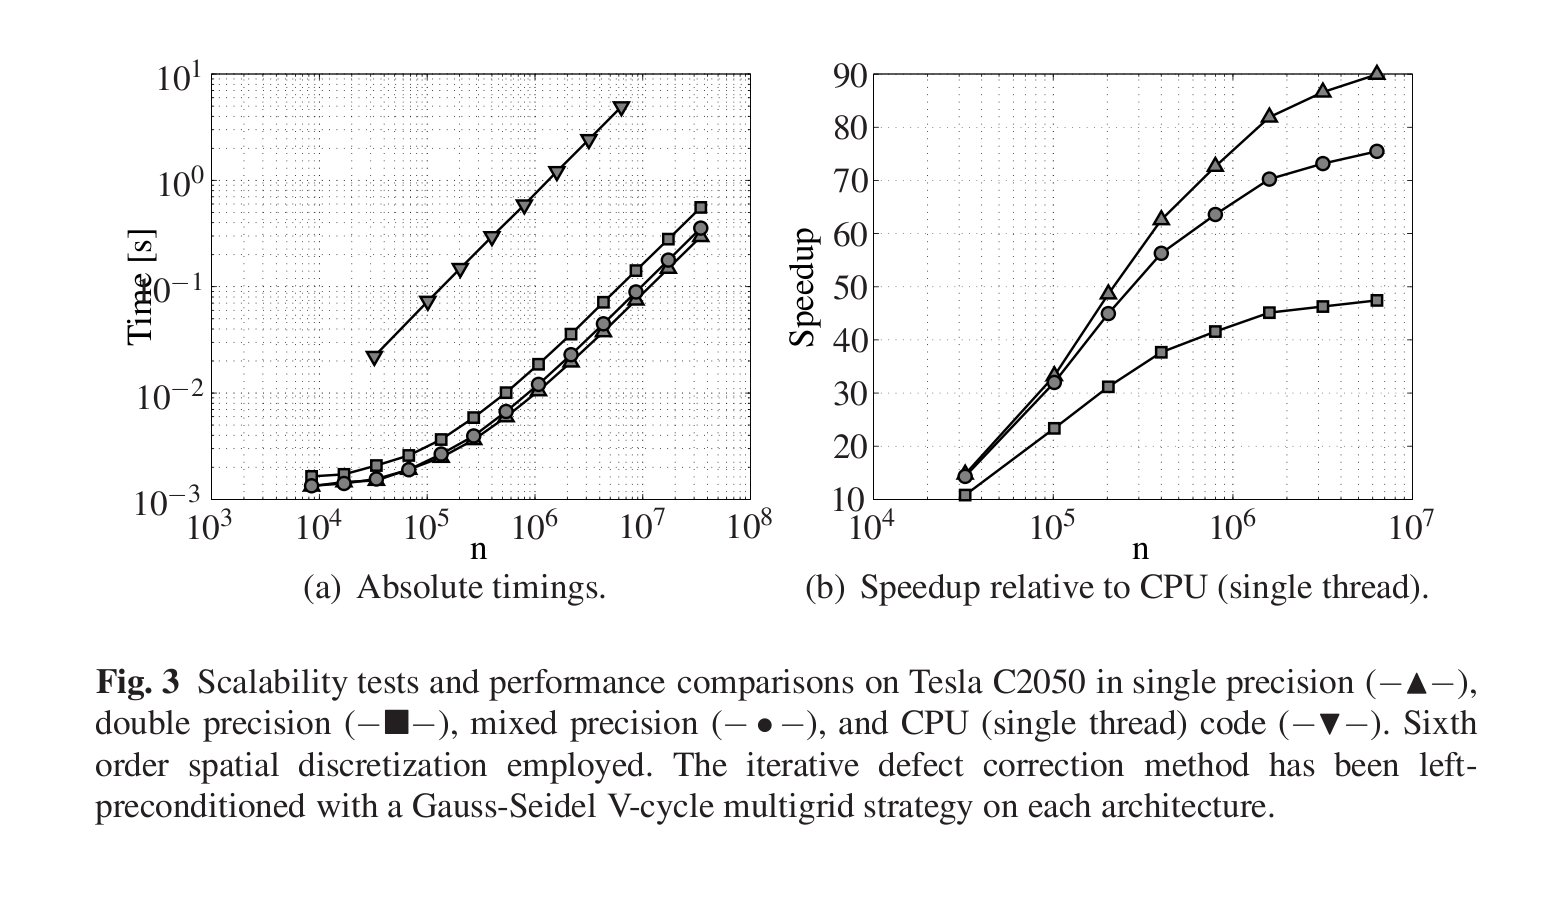
\includegraphics[width=0.9\textwidth]{../SourcesCites/past.jpg}
  %\cite{WaterWaveComp}
  In the year 2013. M. Madesen, S. L. Glimberg and A. P. Engsig-Karup were able to
  achieve a \color{red}38\% performance increase \color{black} using GPU accelerated mixed precision 
  algorithms for full nonlinear water wave computation.\cite{waterwavecomp}
\end{center}
\end{frame}


%\begin{frame}{A brief history overview}
% 
%\begin{itemize}
% \item[] \textbf{$\rightarrow$ Logscale} makes the performance benefits look smaller than they actually are\\
% \item[] \textbf{$\rightarrow$} \color{red} 38\% performance increase\color{black}
%\end{itemize}
%\end{frame}


%\subsection{Performance Gains}
%\begin{frame}{Performance Gains}
%\begin{itemize}
%\item \textbf{Bandwidth bound algorithm}
%	\begin{itemize}
%	\item 64 bit = 1 double = 2 floats = 4 halfs
%	\item More variables per \color{red}{bandwidth}\color{black}
%	\item More variables per \color{red}{storage}\color{black}
%	\item Applies to all memory levels: network, disc, main, device, 
%			local, register
%	\end{itemize}
%\item \textbf{Computation bound algorithm}
%	\begin{itemize}
%	\item 1 double addition $\approx$ 2 float additions $\approx$ 4 half 
%			additions (linear)
%	\item 1 double multip. $\approx$ 4 float multip. $\approx$ 16 
%			half multip. (quadratic)
%	\item $\rightarrow$ up to 16 times better computational efficiency
%	\end{itemize}
%\end{itemize}
%\end{frame}
\section{Floating point operations}
\subsection{Precision}
\begin{frame}{Roundoff and Cancellation}
\onslide<1->
\begin{block}{Definition Machine Precision}
The smallest positive number $\epsilon$ for wich a floating point 
calculation evaluates the expression $1 + \epsilon > 1$ to be true.
\end{block}
\onslide<2->
\textbf{Examples:}
\begin{itemize}
\item $\epsilon_{double} \approx 2.220446049250313\cdot 10^{-16}$
\item $\epsilon_{float} \approx 1.1920929\cdot 10^{-7}$
\item $\epsilon_{half} \approx 9.765625\cdot 10^{-4}$
\item So \color{red}more precision\color{black}~is usually \color{red}better
\end{itemize}
\onslide<3->
\textbf{Examples for cancellation effects in float}
\begin{align*}
&\text{additive roundoff } & a=1+0.00000004 &= 1.00000004 &=_{fl} 1\\
&\text{multiplicative roundoff } & b = 1.0002 \cdot 0.9998 &=0.99999996 &=_{fl} 1\\
&\text{cancellation}  &c\in \lbrace a,b\rbrace 
\hspace{1cm}\pm 4 &= (c-1)\cdot 10^8 &=_{fl} 0 \\
&\text{order~of~operations}  & 1+0.00000004 -1 &=_{fl} 0\\
& &1-1 + 0.00000004 &=_{fl} 0.0000004
\end{align*}
\end{frame}

\subsection{Computational precision vs accuracy of result}
\begin{frame}{Computational precision vs accuracy of result}
\onslide<1->
\begin{block}{Instructive Example [S.M. Rump, 1988]}
$f(x,y) = (333.75 - x^2)y^6 + x^2(11x^2y^2 - 121y^4-2) + 5.5y^8 + 0.5x/y$\\
$x_0 = 77617, y_0 = 33096$
\end{block}

\begin{align*}
&\text{float s23e8} \hfill &1.1726\\
&\text{double s52e11} \hfill &1.17260394005318\\
%&\text{quad s63e15} \hfill &1.172603940053178631
%&\text{quad s112e15} \hfill &1.172603940053178631
\end{align*}
\onslide<2->
\textbf{The correct result is:}\\
\begin{center}
\color{red}-0.82739605994682136814116509547981629\color{black}
\end{center}
\end{frame}

%\subsection{Data Error and Truncation}
%\begin{frame}{DataError and Truncation}
%\begin{itemize}
%\item Data error occurs when the \color{red} exact value~\color{black} has to be \color{red} truncated \color{black} for storage in the binary format%
%	\begin{itemize}
%		\item $\pi$ , $\sqrt{2}$, $sin(2)$, $e^2$, $1/3$
%		\item every rational number with a denominator that has a prime 
%		      factor other than $2$
%	\end{itemize}
%\item How can float be better than double?
%\begin{itemize}
%	\item There is \color{red} no data error \color{black} in the operands
%	\item The errors can \color{red} cancel out \color{black} themselves 
%		  favorably
%\end{itemize}
%\color{black}
%\end{itemize}

%\end{frame}


\subsection{Floting point operations. A deeper analysis}
\begin{frame}{Floting point operations. A deeper analysis}
\textbf{Number representation}\textbf{$\rightarrow$ almost all numbers have to be truncated}~\\
\begin{table}[H]
 \centering
      \begin{tabular}{l|l|l|l}
	half s10e5~a&\text{1 bit sign $s_a$~}&\text{10 bit mantissa $m_a$~}&\text{5 bit exp. $e_a$}\\\hline
	float s23e8~b&\text{1 bit sign $s_b$~}&\text{23 bit mantissa $m_b$~}& \text{8 bit exp. $e_b$}\\\hline
	double s52e11~c&\text{1 bit sign $s_c$~}&\text{52 bit mantissa $m_c$~}&\text{11 bit exp. $e_c$} 
      \end{tabular}
      %\label{tab:L2-Fehler bei einfachen Dimension-Splitting}
\end{table}

\begin{table}[H]
 \centering
      \begin{tabular}{l||l|l}
	\textbf{multiplication} & & \\\hline\hline
	precision & exact format & mantissa truncation: \\\hline\hline
	half(a) $\cdot$ half(b)& s20e6& from 20 to 10 bit \\\hline
	float(a) $\cdot$ float(b)& s46e9& from 46 to 23 bit \\\hline
	double(a) $\cdot$ double(b)& s104e12& from 104 to 52 bit 
      %\label{tab:L2-Fehler bei einfachen Dimension-Splitting}
      \end{tabular}
    \hfill
  \begin{tabular}{l||l|l}
	\textbf{addition} & & \\\hline\hline
	precision & exact format & mantissa truncation: \\\hline\hline
	half(a) + half(b)& s41e5& from 41 to 10 bit \\\hline
	float(a) + float(b)& s278e8& from 278 to 23 bit \\\hline
	double(a) + double(b)& s2099e11& from 2099 to 52 bit 
      %\label{tab:L2-Fehler bei einfachen Dimension-Splitting}
    \end{tabular}
\end{table}

\end{frame}


\section{Example calculation}
\subsection{Algorithm}
\begin{frame}{Algorithm}{mixed precision iterative refinement}
 \begin{algorithm}[H]
  \begin{algorithmic}[1]
    \WHILE{$\Vert r_{m-1} \Vert \cdot \Vert r_0 \Vert ^{-1} > TOL$}
    \STATE{$ r_{m}^h = b - Ax_m$} 
    \STATE{$ r_{m}^l = r_{m}^h$ \textit{\hspace{1cm}//convert from high to low precision}}
    \STATE{$ Ad_{m}^l = r_{m}^l$ \textit{\hspace{1cm}//solve using a fixed number of iterations}}
    \STATE{$ d_m^h = d_m^l$ \textit{\hspace{1cm}//convert from low to high precision}}
    \STATE{$x_{m+1} = x_m + d_m$}
    \ENDWHILE
  \end{algorithmic}
\caption{mixed precision iterative refinement}
\label{alg:seq}
\end{algorithm}
\begin{itemize}
 \item Mixed precision iterative refinement deals with the truncation errors of lower precision data formats
 \item The optimal number of inner iterations was empirically determined

\end{itemize}

\end{frame}


\subsection{Problem definition}
\begin{frame}{Problem definition and Hardware configuration}
\begin{block}{Problem}
Solve the Poission problem $- \Delta u = 1,~x\in\Omega$ with dirichlet boundary conditions $u \equiv 0,~x\in \partial \Omega$ using conforming quadrilateral 
elements for the finite-element discretization of the unit square $\Omega = 
(-1,1)^2$
\end{block}

\begin{itemize}
\item Method 1: Using a V-cycle MG Solver
\item Method 2 : Using a V-cycle MG Solver inside of an iterative refinement loop
\end{itemize}

\begin{itemize}
 \item Hardware configuration 1: i5 2500 + 980Ti \\$\rightarrow$representing a high preformance convetional setup
 \item Hardware configuration 2: Tegra K1 \\$\rightarrow$ representing alternative computing hardware
\end{itemize}



\end{frame}

\subsection{Testresults}
\begin{frame}{Testresults - Accuracy}
 \begin{center}
  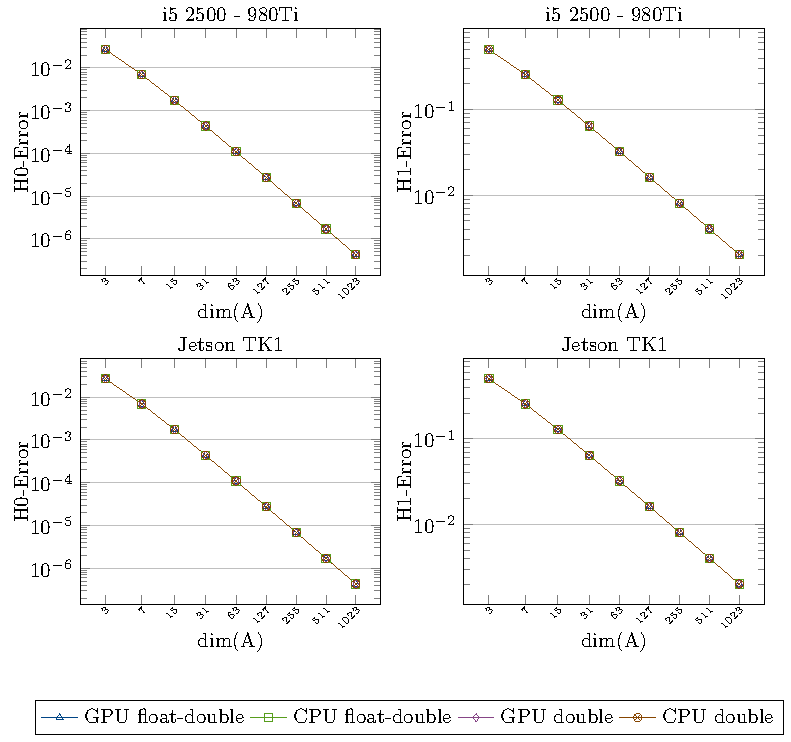
\includegraphics[width=0.6\textwidth]{figures/z-plots2.pdf}
 \end{center}

\begin{itemize}
 \item (virtually) same accuracy as double calculation
 \item H0-Error is $O(m^2)$, H1-Error is $O(m^1)$. [$V_h = Q_1$]
\end{itemize}
\end{frame}

\begin{frame}{Testresults - Performance on comodity Hardware}
  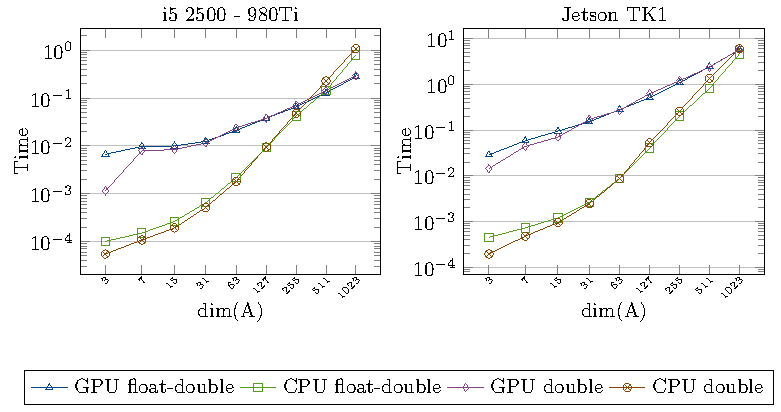
\includegraphics[width=\textwidth]{figures/z-plots3.pdf} %CPU Arryn | GPU Arryn
  \begin{itemize}
 \item \textbf{\color{red} up to 57\%} increase in performance on x86
\end{itemize}
\end{frame}


\begin{frame}{Testresults - Performance on the Tegra K1}
\begin{center}
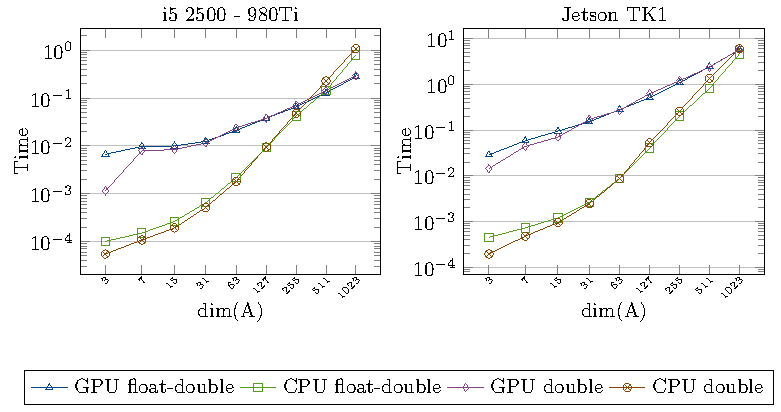
\includegraphics[width=\textwidth]{figures/z-plots3.pdf} %Jetson CPU | Jetson GPU
\end{center}
\begin{itemize}
 \item \textbf{\color{red} up to 65\%} increase in performance on a Jetson TK1
 \item \textbf{ $\rightarrow$ Speedup of about \color{red} 1.6}
 \item \color{black} $\rightarrow$ performance model show that a speedup of 2 is optimal 
 \item \color{black} $\rightarrow$ for longer calculations a speedup of 1.6 can save multiple days
\end{itemize}
\end{frame}

\begin{frame}{Testresults - Half}
\begin{center}
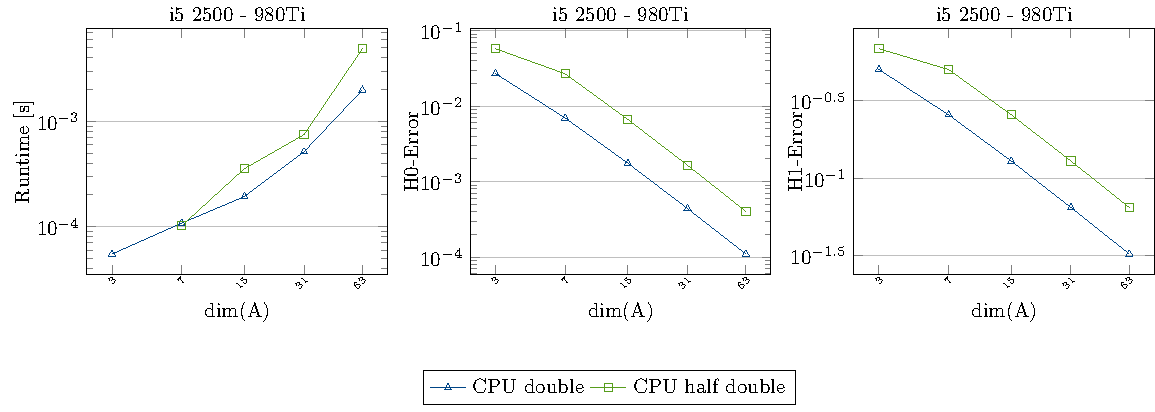
\includegraphics[width=\textwidth]{figures/z-plots4.pdf}
\end{center}
\begin{itemize}
 \item Accuracy loss. Inner solver diverges at more than $63^2$ DOF's.
\end{itemize}
\end{frame}


\begin{frame}{Discussion and Future work}
 \textbf{Future work}
 \begin{itemize}
  \item Try combining half, float and double precision in order to achieve an even greater performance increase
  %\item Use half precision on GPU
 \end{itemize}
 
 \vfill
 \begin{center}
  Thank you for your attention!
 \end{center}

\end{frame}

\begin{frame}{Bibliography}
 \bibliography{literaturscout24.bib}
 \bibliographystyle{plain}
\end{frame}

\end{document}